%file included in thesis.tex


\chapter{Sensors}
\label{chap3-sensors}

\section{Comparisons Between the Proposed Sensors}
For this project, some of the sensors was not decided. This gave the ability to chose a
sensor, based on cost, resolution, accuracy and delivery date. The manufacturers that were
considered where the Japanese \emph{Hokuyo} and American \emph{SICK}. This two companies are to the
authors knowledge the leading manufacturers of laser range finders, small enough to be
mounted on small robotic platforms. The various models and key parameters are summarized
in Table \ref{chap3:tab-sensors}.
\begin{table}[htbp]
    \begin{tabular}{|c|c|c|c|c|c|}
        \hline
        Sensor              & LMS-100 & LMS-200 & UTM-30LX & URG-04LX & URG-04LX-URG01 \\
        \hline
        Max Range           & 20 m    & 80 m    & 30 m     & 4 m      & 5.6 m          \\
        Accuracy            & 12 mm   & 30 mm   & 30 mm    & 10 mm    & 30 mm          \\
        Field-of-View       & $270^\circ$ &$180^\circ$  & $270^\circ$ & $240^\circ$ & $240^\circ$  \\
        Angular Resolution  & $0.25-0.5^\circ$  & $0.25-1^\circ$ & $0.25^\circ$ & $0.36^\circ$ & $0.36^\circ$  \\
        Scan Frequency      & 50 Hz   & 75 Hz   &  40 Hz   & 10 Hz    & 10 Hz          \\
        Weight              & 1.1 Kg  & 4.5 Kg  & 210 g    & 160 g    & 160 g          \\
        Power Consumption   & Not Specified & Not Specified  & $<8 $ W & $~2.5$W  &$~2.5$W  \\
        \hline
        Cost                & \$5500  & \$5000  & \$5000   & \$2400   & \$1100         \\
        \hline
    \end{tabular}
    \caption{Comparison between the proposed sensors}
    \label{chap3:tab-sensors}
\end{table}

The LMS-100 and LMS-200 are relatively large sensors compared to the ones from Hokuyo. The
scanning frequency of the SICK range finders are quicker, but because PiKo is not that
fast and taken into account that the 3D sensor which will have much greater scanning
frequency. This means that the frequency of the 2D sensor is not that important. The most
important thing is that it is as accurate as possible. Also, the Hokuyo sensors are much
cheaper than the ones from SICK which gives them the advantage.

Because of favourable size, weight, accuracy and cost the Hokuyo \emph{URG-04LX} was
chosen. The sensor will be discussed in Section \ref{chap3:sec-urg}.

\subsection{3D Sensors}
There are many different depth sensors available at the consumer market. This section will
outline some of them, and describe the \emph{MESA Imagining} SR-3000 in more detail.
The development of depth-sensing cameras and devices have accelerated the last years
because of the increased computational ability and the fact that electronics become
cheaper and cheaper. \cite{low-cost-depthcameras}

During the next years the video game industry most certainly will
incorporate this new technology into video games to take the games to a new level, such as
Microsofts \emph{Project Natal} for Xbox 360 \cite{project-natal}. This uses infrared
projected light stereo. The camera will sense depth by using stereo cameras to sense a
coded near-infrared light pattern, by using standard CMOS image sensors. According to
Microsoft the accuracy in depth will be about 1 cm, and practical ranges will be about
1 to 3.5 meters. The camera will operate at 640x480 pixel resolution at 60 Hz
\cite{conceivably-tech}.



\section{Laser Range Finder Hokuyo URG-04LX}
\label{chap3:sec-urg}
The laser range finder which were selected to this application was the \emph{Hokuyo
URG-04X}. It uses an infrared laser to sweep a view field of $240^\circ$ ten times a
second. The full $360^\circ$ circle are segmented using ten bit, which gives angular
resolution of $\frac{360}{2^{10}} = 0.3515$. The ranges have twelve bit resolution, each
bit representing a millimeter, which gives the total measurable length of $2^{12} = 4096$.
\begin{figure}[htbp]
    \centering
    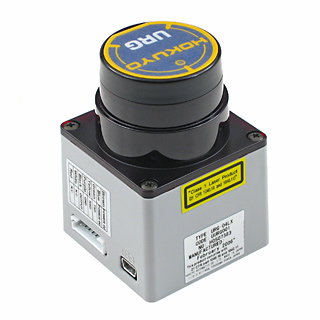
\includegraphics[width=0.4\textwidth]{pics/urg04lx}
    \caption{The Hokuyo URG-04X. \url{http://www.hokuyo.com}}
    \label{chap3:fig-urg}
\end{figure}
The effective area which gives range readings are the sector form the 44th step to
725th step. See Figure \ref{chap3:fig-urg-sector}. If $0^\circ$ is straight ahead, then
the measurement starts at $-135^\circ$ and stops at $135^\circ$. 
\begin{figure}[htbp]
    \centering
    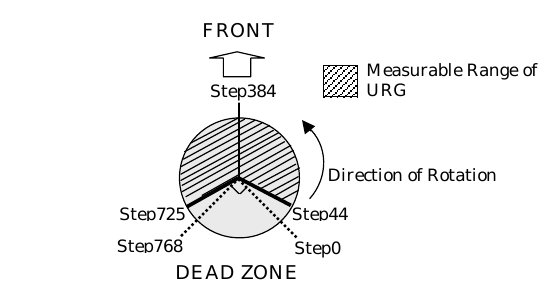
\includegraphics[width=0.7\textwidth]{pics/urg-sector}
    \caption{The sweep sector of the URG-04X}
    \label{chap3:fig-urg-sector}
\end{figure}

The sensor can not measure below 20 mm because it is not practical, and the range codes
from 0--19 are error codes. The codes can describe if the intensity of the reflected light
is too low or too high which indicates erroneous results. A detailed summary of the
error codes and what they mean can be found in Appendix \ref{app:urg-error}.


\subsection{Noise- and Error Sources}
Major error sources of the URG where discussed in Section \ref{chap2:lrf-error}. It is
possible to read both range and intensity of the reflected signal from the URG. The
intensity can be used as a quality control of the range value. 





\section{Stereo Camera Minoru 3D WebCam}
The stereo camera chosen for the project is the first commercially available 3D Webcam.
\begin{figure}[htbp]
    \centering
    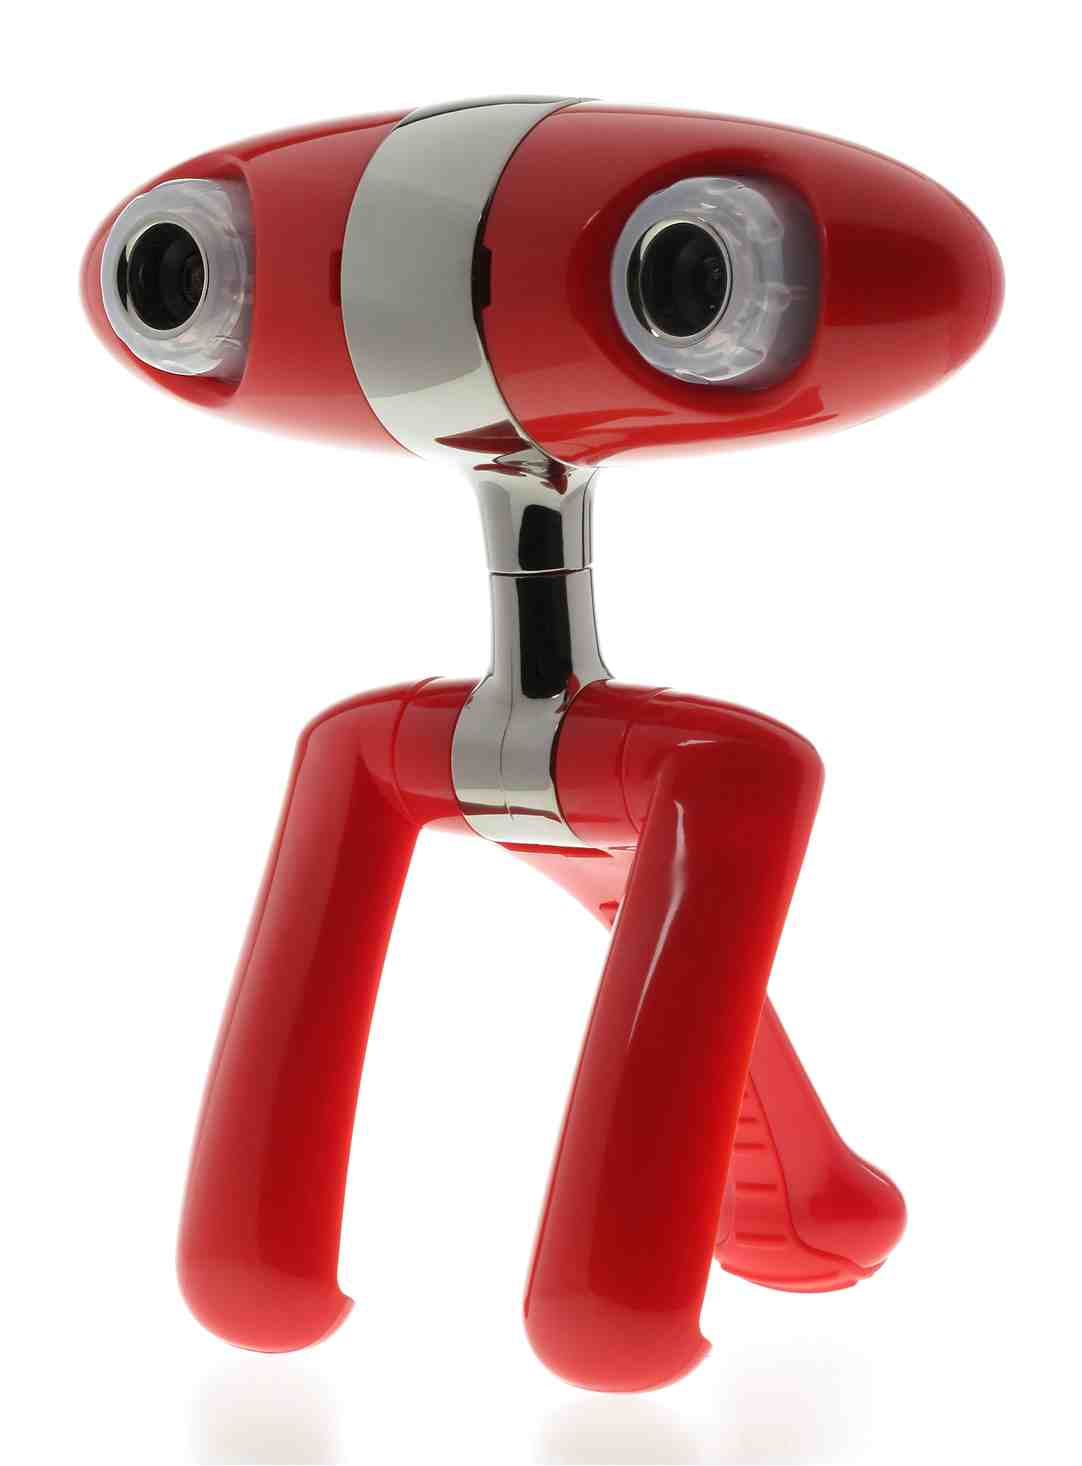
\includegraphics[width=0.35\textwidth]{pics/minoru3d}
    \caption{The Minoru 3D WebCam. \url{www.minoru3d.com}}
    \label{chap3:fig-minoru}
\end{figure}
It is actually just two cheap webcams and a USB hub in the same casing. The camera is
available for about 900 NOK, so both optics and CCD chips are expected to be of poor
quality.


\subsection{Camera Calibration}
To work with stereo images the captured images need to be rectified, i.e. the images need
to be corrected for distortion introduced by the camera lenses. This is a part of
calibrating the camera, meaning that the intrinsic parameters of the camera are
determined and the lens distortion parameters described in Chapter \ref{chap2}.

To determine the parameters the \emph{Camera Calibration Toolbox} for Matlab is used
\cite{camera-calib-toolbox}. 20 image pairs are captured of a checker board in various
distances and orientation from the stereo rig. This images for left and right camera are
processed individually to calculate the distortions of the individual camera. 
\begin{figure}[htbp]
    \centering
    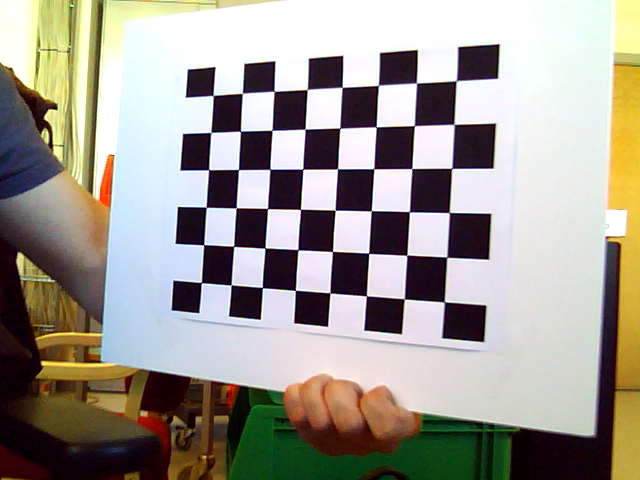
\includegraphics[width=0.8\textwidth]{pics/left7}
    \caption{Seventh left image in the calibration sequence}
    \label{chap2:fig-checkerboard}
\end{figure}
The four extreme-most corners of the checkerboard is selected in each image, and an
internal algorithm detects the corners of the squares in each image. This gives an initial
guess on how the distortion parameters are. The reprojection error is then minimized with
regard to the distortion parameters using a nonlinear gradient decent algorithm. For more
information on how this is carried out, see \cite{heikkila}.

The distortion parameters for both cameras are summarized in Table
\ref{chap3:tab-distortion-coeffs}.
\begin{table}[htbp]
  \centering
    \begin{tabular}{|c|c|c|} 
        \hline
                & Left Camera       & Right Camera \\
        \hline
        $k_1$   & $-0.10292 \pm 0.3794$            & $-0.5450 \pm 0.02456$  \\
        $k_2$   & $-0.22555 \pm 0.49387$            & $-0.38334 \pm 0.13037$  \\
        $h_3$   & $ 0$                          & $0$                  \\
        \hline
        $p_1$   & $-0.00361 \pm 0.00141$    & $-0.00033 \pm 0.00115$ \\
        $p_2$   & $0.00206 \pm 0.00174$     & $ 0.000491 \pm 0.00243$  \\
        \hline
    \end{tabular}
    \caption{The distortion parameters discussed in Section \ref{chap2:sec-distortion}}
    \label{chap3:tab-distortion-coeffs}
\end{table}





Figure \ref{chap3:fig-comp-lensdist} below shows how the camera lenses of the Stereo camera distorts the pictures
towards the edges of the lens. 
\begin{figure}[htbp]
    \centering
    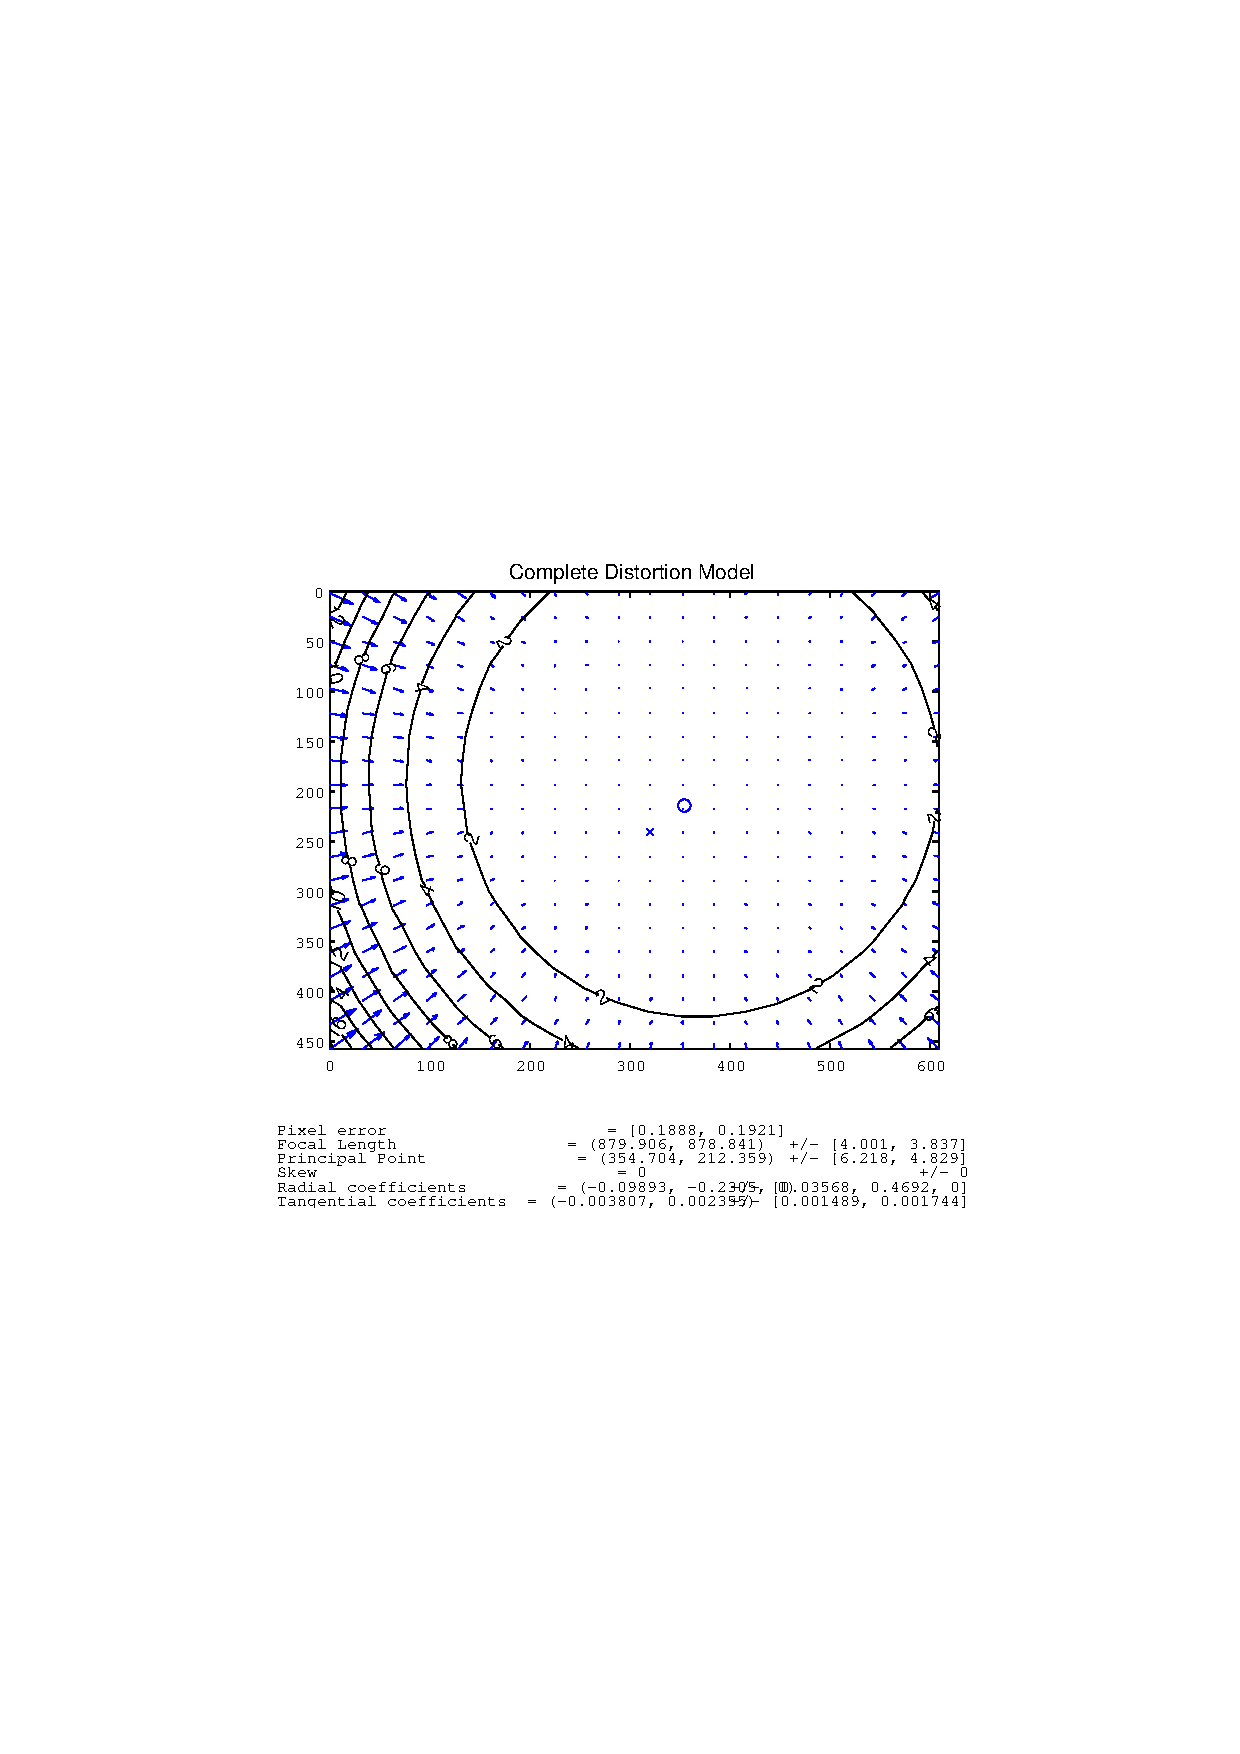
\includegraphics[width=0.47\textwidth]{pics/left_comp_dist}
    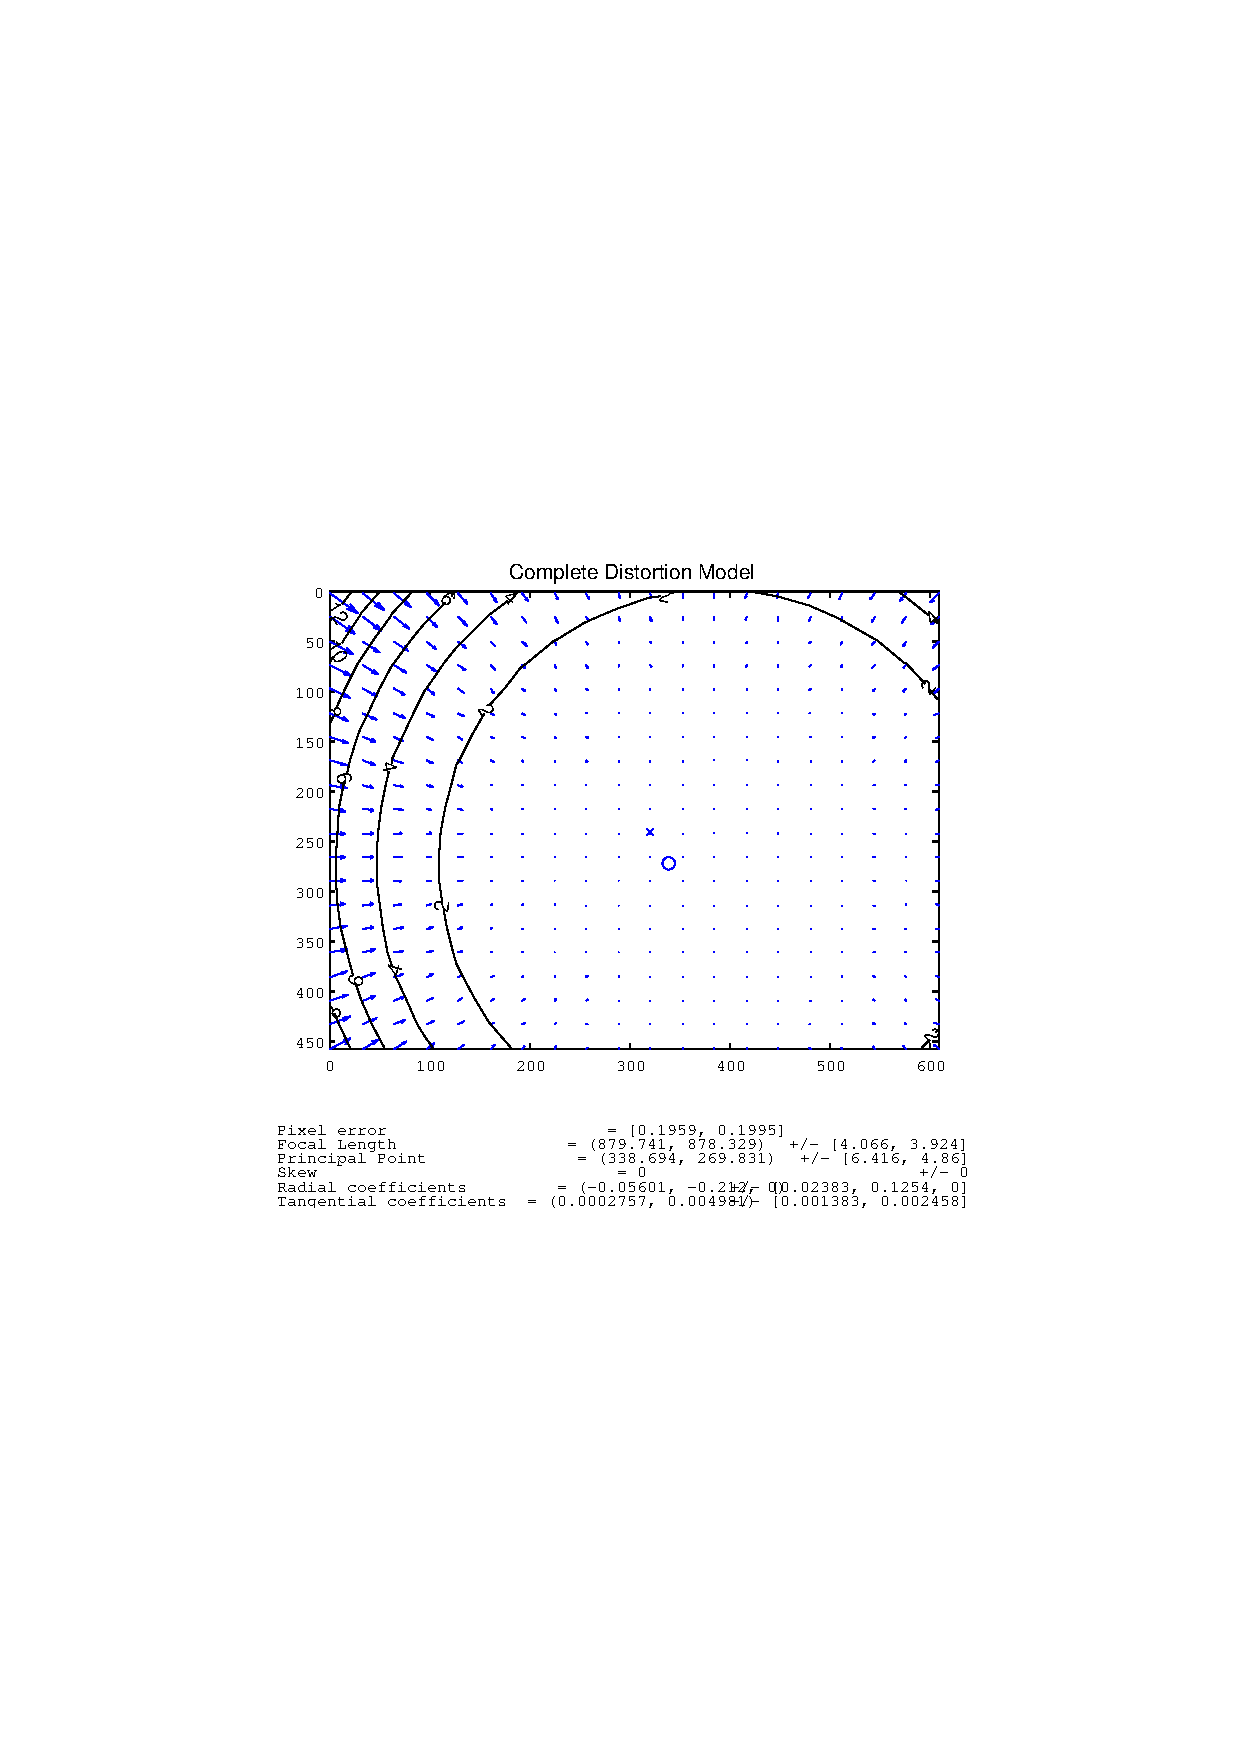
\includegraphics[width=0.47\textwidth]{pics/right_comp_dist}
    \caption{The left and right camera distortion due to lens nonlinearities}
    \label{chap3:fig-comp-lensdist}
\end{figure}
The Figure clearly shows that the principal axis are offset from the center of the images,
and that it is opposite for the left and right images. This means that the view field of
the two cameras will be quite different, and result in a reduced field-of-view for the
total stereo rig.

The intrinsic parameters for the cameras are summarized in Table
\ref{chap3:tab-intrinsic-stereo}. The values are all in pixel coordinates. The real focal
distances can be calculated by knowing the pixel-to-length ratio.
\begin{table}[htbp]
  \centering
    \begin{tabular}{|c|c|c|} 
        \hline
                & Left Camera       & Right Camera \\
        \hline
        $f_x$   & $877.11\pm 2.94$  & $880.28\pm 3.08$  \\
        $f_y$   & $876.49\pm 2.88$  & $879.20\pm 2.96$  \\
        \hline
        $c_x$   & $350.00\pm 6.32$  & $338.54\pm 6.21$ \\
        $c_y$   & $214.30\pm 4.65$ & $267.59\pm 4.35$  \\
        \hline
    \end{tabular}
    \caption{Intrinsic parameters of the stereo rig in pixel related units including
    uncertainties}
    \label{chap3:tab-intrinsic-stereo}
\end{table}
The focus distances in the x and y-direction are slightly different in both cameras. This
suggests that the pixels of two cameras are not exactly square. The principal axis in both
cameras are also in very different places. This is problematic because a stereo rig should
be horizontally aligned to give the best results. Because for the off-center principal
axis the field-of-view of the stereo rig will be quite reduced.


This distortion can be removed and are called rectifying the image. This makes common
features in the two images aligned horizontally. This makes it much easier for the matching
algorithm because it only need to match vertically.


\subsection{Depth resolution}
The depth resolution which can be expected from the Stereo cam are,
\begin{equation}
    \Delta Z = \frac{Z^2}{f T}\Delta d
\end{equation}
where $\Delta d$ is the smallest increment in disparity, $f$ is the focal distance, and
$T$ is the baseline. This is determined in the implementation in this case the OpenCV
library. This is useful when calibrating the stereo rig, and when testing the program,
because it tells what kind of ranges one can expect from the rig.


\subsection{Noise- and Error Sources}
The major source of errors connected with stereo cameras are bad feature matches. This
will cause bogus distances. This is heavily correlated with the amount of noise captured
by the imaging sensors and other disturbances.




\section{Time-of-Flight Camera MESA SwissRanger-3000}
The 3D sensor chosen for the project is the MESA SwissRanger-3000 Time-of-Flight Camera.
This is based on amplitude modulation of near-infrared light (850 nm), which is emitted from an
array of 55 LEDs and captured at a spherical PMD chip. The spatial resolution of the camera
are $176\times144$ with a field-of-view of $47.5^\circ \times 39.6^\circ$. 
\begin{figure}[htbp]
    \centering
    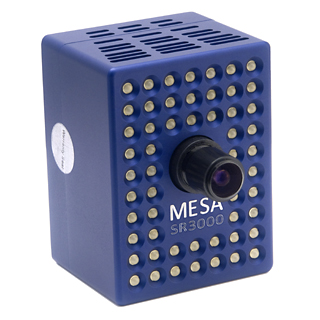
\includegraphics[width=0.4\textwidth]{pics/sr3000}
    \caption{The SwissRanger-3000 Time-of-Flight Camera. \url{http://www.mesa-imaging.ch}}
    \label{chap3:fig-sr3000}
\end{figure}
The amplitude modulation frequency are set to 20 MHz which gives a non-ambiguity range of
7.5 meters. If the modulation frequency is lowered the maximum measured distance might be
larger, but this distance is good for the application of the project. 

Since the camera needs lots of cooling because of the LEDs and electronics the camera are
mounted on a stem of aluminium, to secure the airflow through the camera. 

The camera outputs standard Cartesian coordinates or spherical coordinates and the
intensity, which is comparable to a standard gray scale camera. Figure 
\ref{chap3:fig-tof-amppicture} shows a typical amplitude plot of the inside of a pipe.
\begin{figure}[htbp]
    \centering
   % 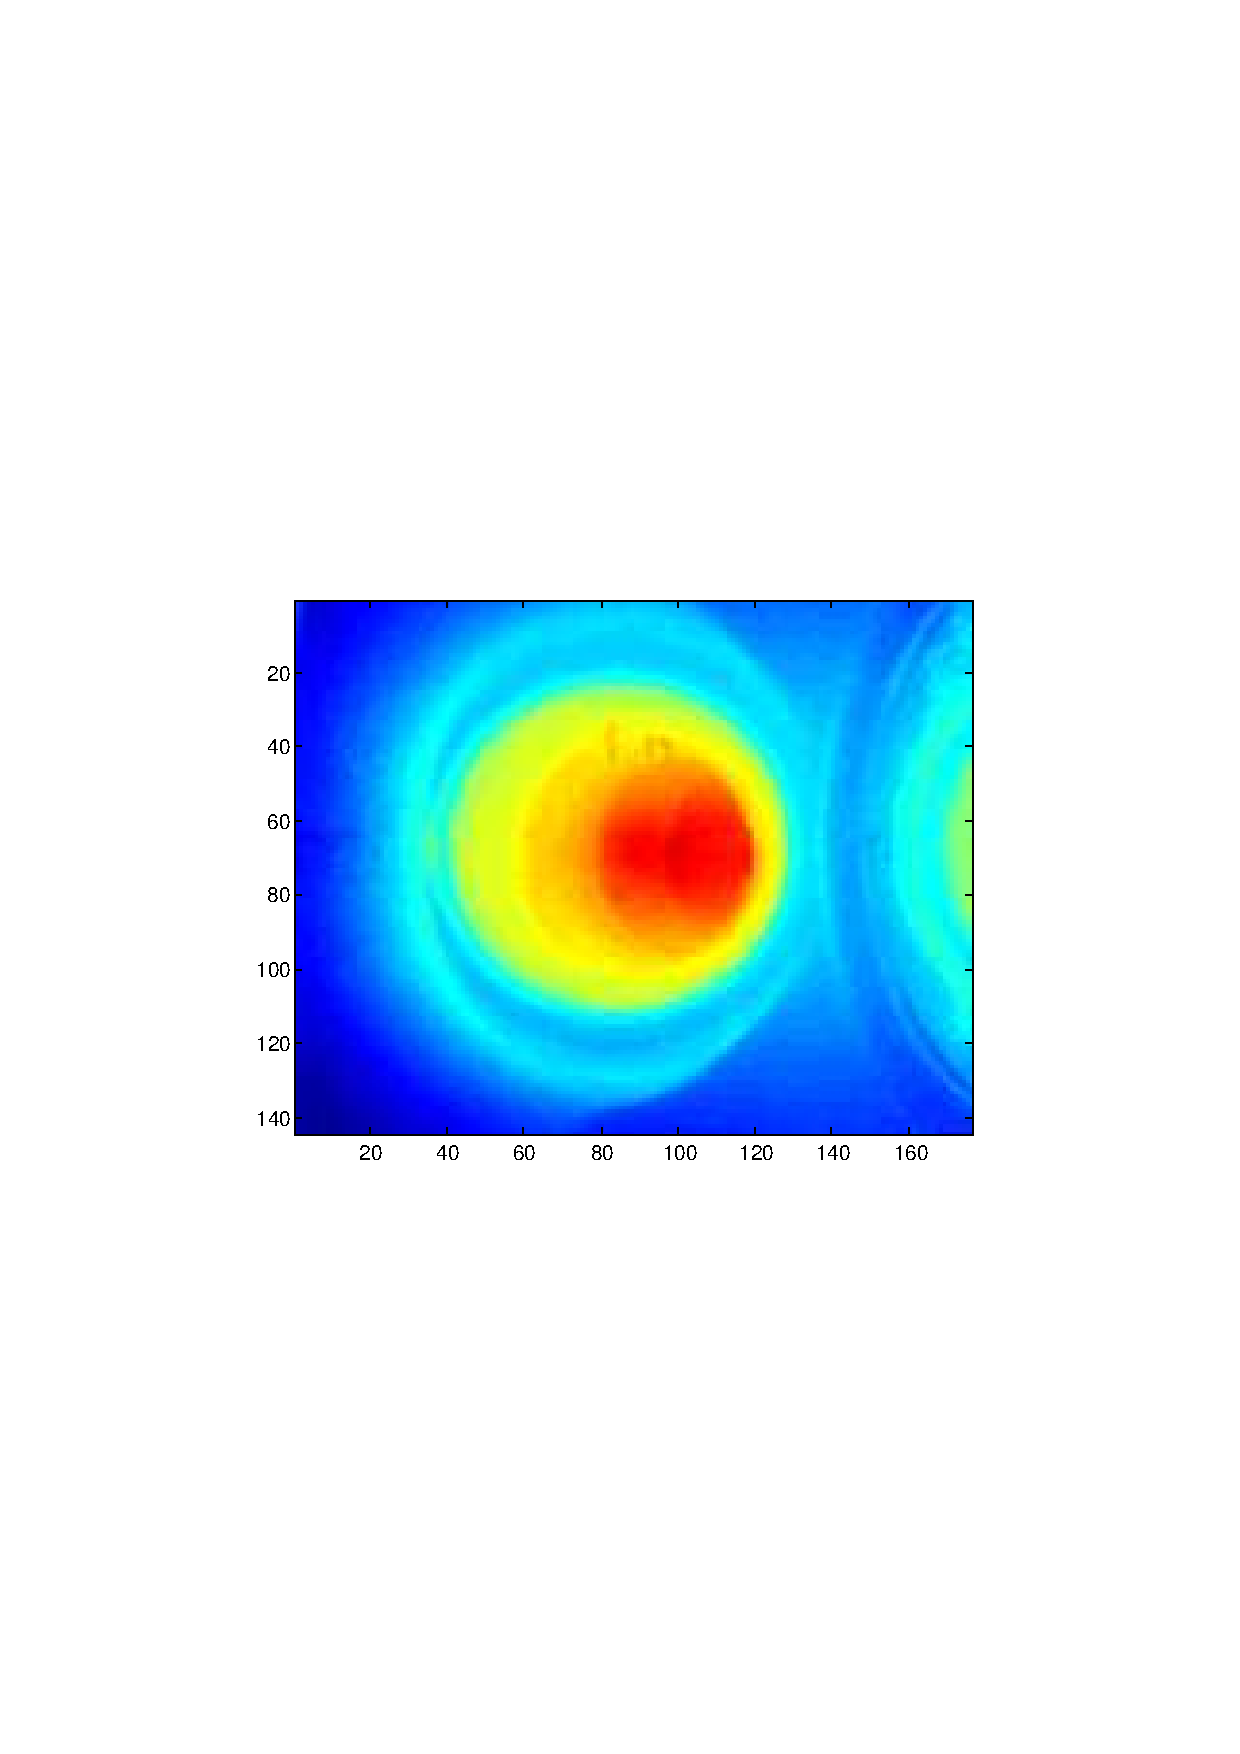
\includegraphics[width=0.8\textwidth]{pics/tof-amppicture}
    \caption{Typical amplitude image of the SR-3000 ToF-camera}
    \label{chap3:fig-tof-amppicture}
\end{figure}


\subsection{Intrinsic Parameter Calibration}
The intrinsic parameters are determined the same way as for the individual cameras in the
stereo rig. This is to determine the lens distortions and principal axis, see Table
\ref{chap3:tab-intrinsic-sr3000}.
\begin{table}[htbp]
  \centering
    \begin{tabular}{|c|c|c|} 
        \hline
                & SR-3000       & Given by Manufacturer \\
        \hline
        $f_x$   & $212.52 \pm 14.91 $  & $200$  \\
        $f_y$   & $213.94 \pm 14.96 $  & $200$  \\
        \hline
        $c_x$   & $88.63 \pm 5.00$  & $88$ \\
        $c_y$   & $ 62.96 \pm 5.67 $ & $72$  \\
        \hline
    \end{tabular}
    \caption{Intrinsic parameters of the ToF-camera in pixel related units including
    uncertainties}
    \label{chap3:tab-intrinsic-sr3000}
\end{table}
The focal distances given from the manufacturer are calculated using the pixel size of
$40 \times 40 \mu m^2$ and 8 mm focal distance.

The calibration method is the same as for the stereo cameras. The intensity images from
the camera are captured, converted to 8-bit integer values and histogram normalized to
enhance give better contrast. This makes the finding of the checkerboard corners easier in
the calibration process. Since the spatial resolution of the camera are small, noise and
inaccurate sampling make the corner selection problematic. This shows itself on the large
uncertainties int in the focal distances. 

\begin{figure}[htbp]
    \centering
    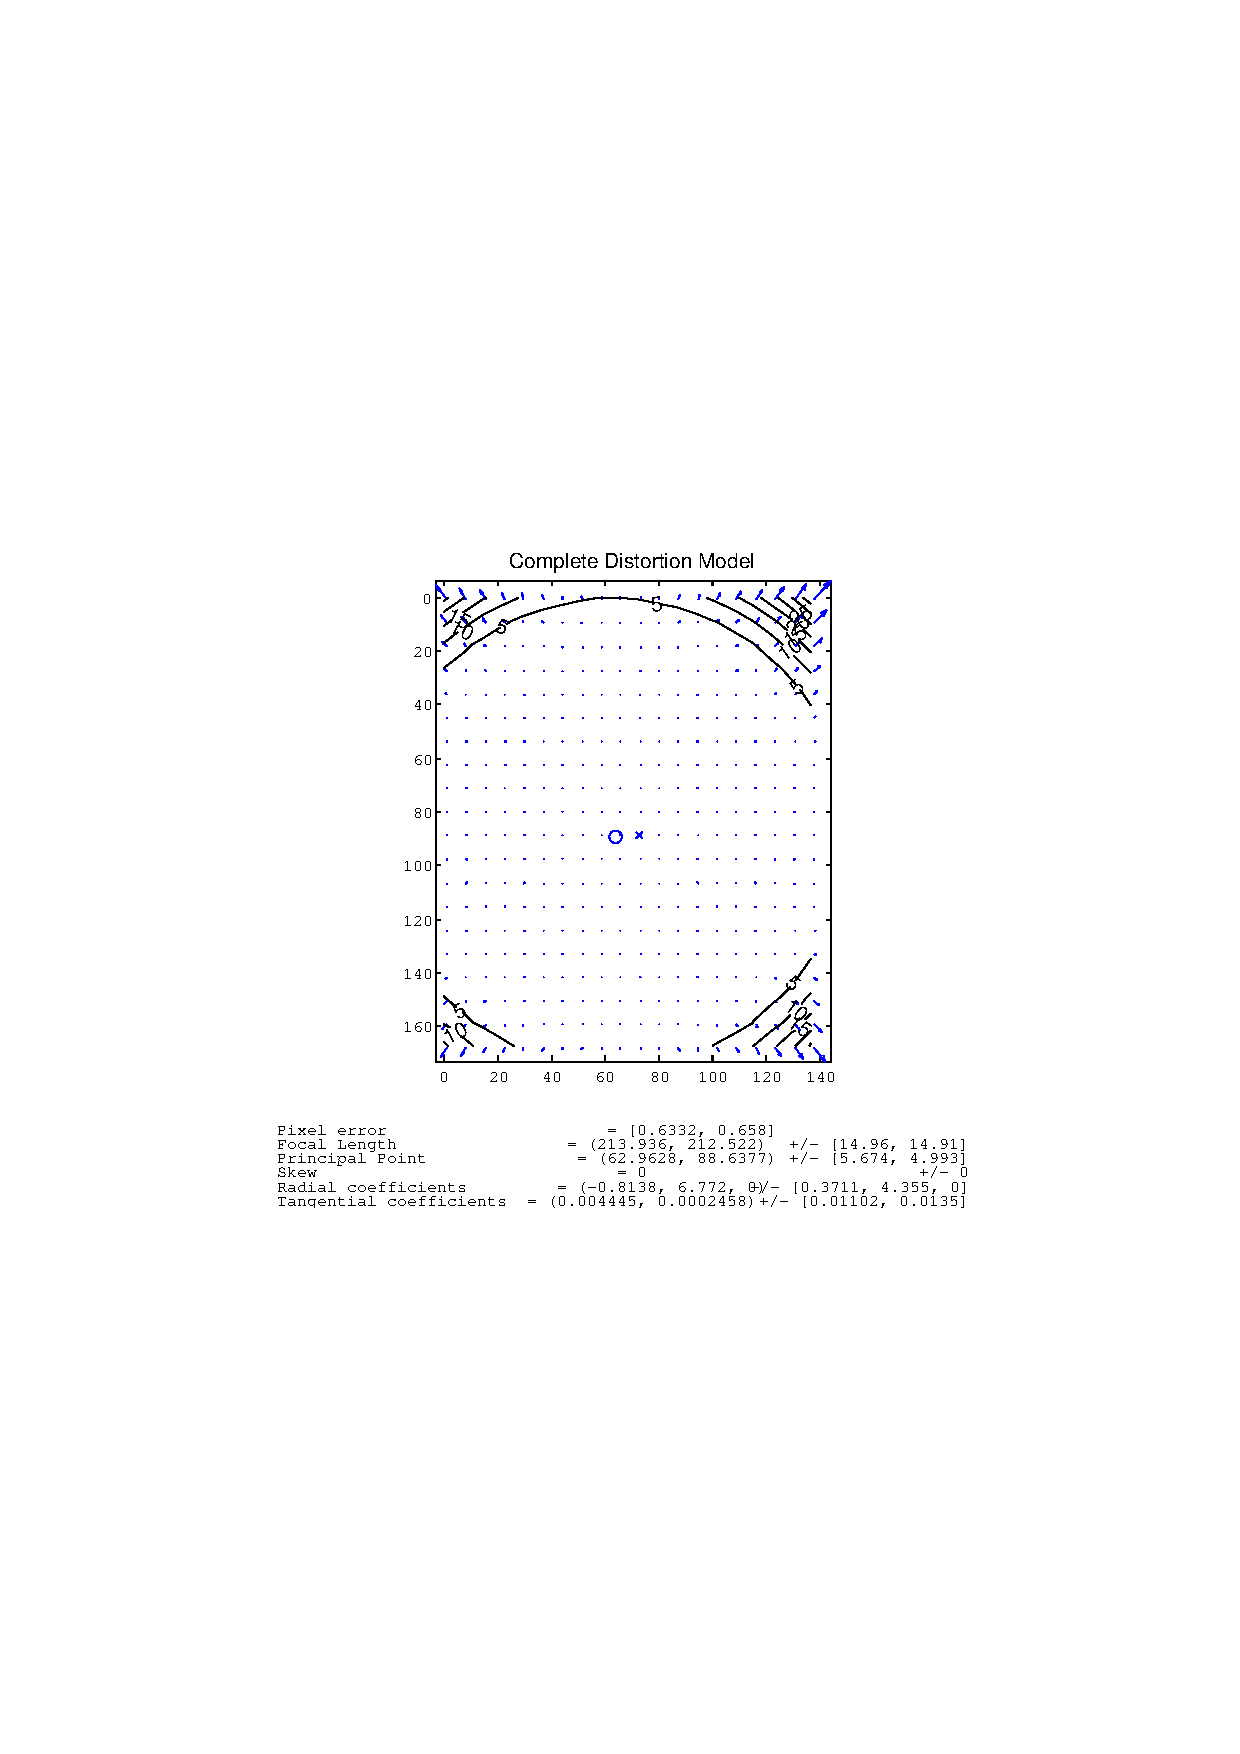
\includegraphics[width=0.7\textwidth]{pics/sr3000_comp_dist}
    \caption{The lens distortion for SwissRanger 3000}
    \label{chap3:fig-sr3000-comp-lensdist}
\end{figure}
From the Figure \ref{chap3:fig-sr3000-comp-lensdist} the distortion due to lens are shown.
The principal axis are off center in the y-direction, this might be the case, but can also
be inaccuracies caused by the calibration. 



\subsection{Depth Calibration}




\subsection{Noise- and Error Sources}
As stated in Section \ref{chap2:sec-tof} the complete picture of the distances are
captured fist when 4 successive exposures are complete. This means that fast moving
objects will cause distance errors because the object might have moved between the
exposures. Another source of errors are multiple reflections and highly reflective
surfaces which will cause errors because too much light is reflected. The same is the case
with surfaces which absorbs most of the light. This surfaces will appear farther away than
they really are. 





\section{Sensor Configurations}
There are a couple of possible sensor configurations available for this project. ***SHOULD
MAYBE BE IN THE IMPLEMENTATION CHAPTER?****

The Laser Range Finder should alway be used in every sensor configuration. This should be
the primary source of length measurements since this is the most accurate of all the range
devices. 

The stereo camera might be looked upon as a cheap type of the Time-of-Flight camera. So
the two possible configurations are:
\begin{itemize}
    \item Laser Range Finder and Stereo Camera
    \item Laser Range Finder and Time-of-Flight Camera
\end{itemize}
The Stereo Camera will give sparse range data, while the Time-of-Flight camera will give
dense range data. 




